\documentclass[12pt, a4paper, twocolumn, twoside]{article}

\usepackage[top=2cm, bottom=2cm, left=3cm, right=3cm]{geometry}
\usepackage{lipsum}
\usepackage{graphicx}
\usepackage[english, russian]{babel}
\usepackage{tempora}            % TNR для кириллицы
\usepackage{amsmath}            % мат. окружение align
\usepackage{amssymb}            % мат. символы
\usepackage{fancyhdr}           % колонтитулы
\usepackage{multirow}
\usepackage{caption}
\usepackage{array}
\usepackage{xcolor}
\usepackage{hyperref}


\setcounter{page}{14}

\fancyhf{}
\fancyfoot[LE,RO]{\textbf{\thepage}}
\pagestyle{fancy}

\setlength{\parindent}{2em}         % красная строка
\setlength{\arrayrulewidth}{0.5mm}  % толщина границ таблицы

\renewcommand{\thefootnote}{\fnsymbol{footnote})\space\space}
\renewcommand{\headrulewidth}{0pt} % убираем линии на колонтитулах
\renewcommand{\footrulewidth}{0pt}



\begin{document}

\onecolumn
\thispagestyle{empty}

{
\fontsize{14pt}{20pt}
\selectfont

\begin{center}
    Федеральное государственное автономное образовательное учреждение высшего образования <<Национальный исследовательский университет ИТМО>> \\
\end{center}

\begin{center}
    \textit{Факультет программной инженерии и компьютерной техники \\ 
    Направление подготовки: 09.03.04 – Программная инженерия, Системное и прикладное программное обеспечение}
\end{center}

\begin{center}
    \textit{Дисциплина: Информатика}
\end{center}

{
\fontsize{16pt}{20pt}
\selectfont
\vspace{3cm}
\begin{center}
    \textbf{\textcolor{red}{Лабораторная работа №6} \\
    Работа с системой компьютерной верстки \TeX} \\
    Вариант №16
\end{center}
}


\vspace{6cm}
\begin{flushright}
    Выполнил: \\
    Карнажицкий Максим Романович \\
    Группа: P3111 \\
\end{flushright}
\begin{flushright}
    Проверил: \\
    Доцент факультета ПИиКТ \\
    Малышева Т. А.
\end{flushright}

\vfill

\begin{center}
    г. Санкт-Петербург, 2024
\end{center}

}
\newpage
\setcounter{page}{14}
\twocolumn

\vspace*{2.5cm}

\noindent \textit{И. Быстрый} \\

\noindent \textbf{\huge Площадь сегмента параболы Нейля}

\vspace{1cm}
\noindent В 1657 году двадцатилетний студент Оксфордского университета Уильям Нейль (1637--1670) нашел длину дуги <<полукубической параболы>> $y=a \sqrt[3]{x^2}$. Это открытие поразило современников, и в память о рано умершем талантливом математике полукубическая парабола называется \textit{параболой Нейля}.

В наше время параболу Нейля можно встретить не только в вузовском курсе анализа, но и в школьном учебнике\footnote{<<Алгебра и начала анализа 9>>, задачи 438, 474б, <<Алгебра и начала анализа 10>>, задача 393а}). А недавно на лекции для абитуриентов я получил такую записку:

\textit{Как найти площадь фигуры, ограниченной кривой $y=3 \sqrt[3]{x^2}$ и касательной к ней в точке $x=-8$?}

Вот что я тогда ответил.

Эта задача, несмотря на кажущуюся простоту, связана с определенными трудностями. Первая трудность возникает при нахождении касательной к параболе Нейля
\vspace{-5pt}
\begin{align}
    f_1(x) &= 3 \sqrt[3]{x^2} \label{eq:f1}
\end{align}
в точке $x=-8$. Как известно, уравнение касательной определяется по формуле
\vspace{-5pt}
\begin{align}
y-f_1(-8)=f_1'(-8)(x+8). \label{eq:f2}
\end{align}
Здесь
\vspace{-10pt}
\begin{align*}
    f_1(-8)=12,
\end{align*}
\begin{align*}
    f_1'(-8) &= 3(x^{\frac{2}{3}})'|_{x=-8} = \\
    &= 3 \cdot \frac{2}{3}x^{- \frac{2}{3}}|_{x=-8}=2\cdot (-8) ^ {- \frac{1}{3}}.
\end{align*}
Значит, производная не существует (поскольку выражение $(-8)^{- \frac{1}{3}}$ не имеет смысла), следовательно, не существует и касательной к кривой (1).

Между тем, из чертежа ясно, что вывод неверен: прямая $(AB)$ -- касательная! В чем дело? Как же найти угловой коэффициент касательной? Дело в том, что формула 
\vspace{-5pt}
\begin{align*}
    (\sqrt[n]{x^m})'=(x^{\frac{m}{n}})'=\frac{m}{n}x^{\frac{m}{n}-1},
\end{align*}
верная при $x \geq 0$, здесь неприменима. Для вычисления производной (при $x<0$) следует пользоваться формулой
\vspace{-5pt}
\begin{align}
    (\sqrt[n]{x^m})'=\frac{m}{n}\frac{\sqrt[n]{x^m}}{x}, \tag{*} \\
    x \neq 0, n \in \mathbb{N}, m \in \mathbb{Z}. \notag
\end{align}
(которая, разумеется, применима и для положительных $x$). В соответствии с ней имеем
\vspace{-5pt}
\begin{align*}
    f_1'(-8)=(3\sqrt[3]{x^2})&'|_{x=-8}=\\
    &=3\cdot\frac{2}{3}\frac{\sqrt[3]{(-8)^2}}{(-8)}=-1
\end{align*}
Подставив $f_1(-8)=12$ и $f_1(-8)=-1$ в равенство (\ref{eq:f2}), получим искомое уравнение касательной 
\vspace{-5pt}
\begin{align*}
    y=4-x.
\end{align*}

У п р а ж н е н и е 1. \textit{Найдите точки пересечения линий $f_1(x)=3\sqrt[3]{x^2}$ и $f_2(x)=4-x$}.

Теперь, когда известна абсцисса точки $B$, легко найти площадь криволинейного треугольника $AOB$.

\vspace{0.5cm}
\begin{figure}[h]
    \centering
    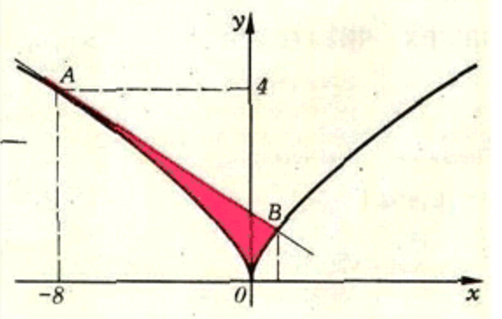
\includegraphics[width=1\linewidth]{latex21111.png}
    \label{fig:enter-label}
\end{figure}
% \newpage
\begin{center}
\begin{table*}[t]
    \captionsetup{justification=raggedleft, singlelinecheck=false, position=above}
    \caption*{Т а б л и ц а}
    \centering
    \small
    \begin{tabular}{|>{\raggedleft}p{2cm} m{0.5cm}  m{0.8cm} m{0.8cm} m{0.8cm} m{0.8cm} m{0.8cm} m{0.8cm} m{0.8cm} c >{\centering\arraybackslash}m{1.3cm}|}
         \hline
          & & & & & & \multicolumn{4}{c}{Продолжительность} & \\
          & & \multicolumn{2}{c}{Восход} & \multicolumn{2}{c}{Заход} & \multicolumn{2}{c}{дня} & \multicolumn{2}{c}{ночи} & \\
           & & ч & мин & ч & мин & ч & мин & ч & мин & Разность мин \\
          \hline
          
          \multirow{7}{*}{Март\vspace{2cm}} & & & & & & & & & & \\
          & 17 & 6 & 41 & 18 & 37 & 11 & 56 & 12 & 04 & --08 \\
          & 18 & 6 & 38 & 18 & 39 & 12 & 01 & 11 & 59 & +02 \\
          & 19 & 6 & 36 & 18 & 41 & 12 & 05 & 11 & 55 & +10 \\
          & 20 & 6 & 34 & 18 & 43 & 12 & 09 & 11 & 51 & +18 \\
          & 21 & 6 & 31 & 18 & 45 & 12 & 14 & 11 & 46 & +28 \\
          & & & & & & & & & & \\

          \hline
          \multirow{7}{*}{Сентябрь\vspace{2cm}} & & & & & & & & & & \\ 
          & 23 & 6 & 16 & 18 & 28 & 12 & 12 & 11 & 48 & +24 \\
          & 24 & 6 & 18 & 18 & 25 & 12 & 07 & 11 & 53 & +14 \\
          & 25 & 6 & 20 & 18 & 22 & 12 & 02 & 11 & 58 & +04 \\
          & 26 & 6 & 22 & 18 & 20 & 11 & 58 & 12 & 02 & --04 \\
          & 27 & 6 & 24 & 18 & 17 & 11 & 53 & 12 & 07 & --14 \\
          & & & & & & & & & & \\
          
          \hline
    \end{tabular}
    \label{tab:table}
\end{table*}
\end{center}

\vspace{-20pt}
Лучи света от небесного тела, прежде чем попасть в глаз наблюдателя, проходят сквозь земную атмосферу, преломляясь в ней, как в призме. Так как плотность атмосферы увеличивается к поверхности Земли, лучи преломляются все сильнее и сильнее по мере приближения к Земле.

\lipsum[1-3]

\fancyhf{}
\fancyfoot[LE,RO]{\textbf{3*\hfill\thepage}}
\pagestyle{fancy}
\newpage

\end{document}